\documentclass{article}

\usepackage[english]{babel} % required to compile for windows
\usepackage[utf8]{inputenc}
\usepackage[T1]{fontenc}
\usepackage{geometry}
\usepackage{listings}
\usepackage{fancyhdr} % header
\geometry{a4paper, left=2cm, right=2cm, top=3cm, bottom=4cm} 

% header
\pagestyle{fancy}
\fancyhead{} % clear header
\fancyfoot{} % clear footer
\setlength{\headheight}{50pt}

\chead{{\large Schnupperuni Informatik}}

\lhead{FOSS-AG}
\rhead{23. - 26.10.2017}
\cfoot{-\thepage-}

\begin{document}
	\begin{center}
		\huge Von Schlangen und Himbeerkuchen:\\Programmieren in der Welt von Minecraft
	\end{center}
	\section{Einführung}
		\large Schreibe ein Python-Script, das dafür sorgt, dass stets Blumen auf dem Block generiert werden, auf dem Steve sich befindet.
Gehe dafür wie folgt vor:
\begin{itemize}
	\item Binde zunächst die Minecraft-Bibliothek ein, um mit dem Spiel zu kommunizieren.
	\begin{lstlisting}[language=Python]
import mcpi.minecraft as minecraft
	\end{lstlisting}
	
	\item Baue die Verbindung zum Spiel auf.
	\begin{lstlisting}[language=Python]
mc = minecraft.Minecraft.create()
	\end{lstlisting}
	Das Objekt \textbf{mc} stellt nun die Kommunikationschnittstelle mit dem Spiel dar.
	
	\item Speichere dir die Block-ID der Blume (38) in einer Variable zwischen. Das erleichtert das Programmieren und macht den Code einfacher zu lesen.
	
	\item Verwende eine \textbf{while}-Schleife für den Hauptteil deines Scripts. Da das Platzieren der Blumen solange stattfinden soll, wie das Spiel läuft, wird eine Schleife benötigt, die nur durch Beenden des Programms abgebrochen werden kann.
	
	\item Frage innerhalb der \textbf{while}-Schleife die aktuelle Position von Steve ab. Diese benötigen wir, um an genau dieser Stelle die Blumen platzieren zu können.
	
	\item Platziere zu guter letzt an Steves aktueller Position die Blumen. 
\end{itemize}
	\section{Shuffle Block}
		\subsection{}
		\large Schreibe ein Python-Script, das dafür sorgt, dass Blöcke, die du mit der rechten Maustaste schlägst, wie unten beschrieben, durchwechseln.
Gehe dafür wie folgt vor:
\begin{itemize}
	\item Ergänze den Code nur in dem gekennzeichneten Rahmen.
	
	\item Die Liste \texttt{block\_list} beinhaltet alle Blöcke, durch die durchgewechselt werden sollen.
	
	\item Lege außerhalb der \texttt{while}-Schleife eine Variable an, die dazu dient, die aktuelle Position in \texttt{block\_list} zu speichern. Somit kannst du dir merken, welcher Block als nächstes gesetzt werden soll.
	
	\item Schreibe innerhalb der \texttt{while}-Schleife eine \texttt{for}-Schleife, die für jeden geschlagenen Block den Schleifenrumpf ausführt. Um die Liste der angeschlagenen Blöcke zu erhalten verwende die Funktion
	\begin{lstlisting}
mc.events.pollBlockHits()
	\end{lstlisting}
		
	\item Ersetze den geschlagenen Block durch den aktuellen Block in \texttt{block\_list}. Nutze dafür die Funktion
	\begin{lstlisting}
mc.setBlock(x_pos, y_pos, z_pos, block_id, 1)
	\end{lstlisting}
	Gehe danach sofort einen Schritt weiter in der Liste.
	
	\item Ist das Ende der Liste erreicht, wird die Liste wieder von vorne durchlaufen.
\end{itemize}
		\subsection{}
		Erweitere den ersten Aufgabenteil wie folgt:
\begin{itemize}
	\item Wird ein Block geschlagen, soll er nicht einfach durch den aktuellen Block in der Liste ersetzt werden, sondern abhängig vom geschlagenen Block behandelt werden. Ist der geschlagene Block nicht in der Liste vorhanden, so wird er durch den ersten Block der Liste ersetzt. Befindet sich der Block in der Liste, so wird er durch den nachfolgenden Block in der Liste ersetzt.
	
	\item Um herauszufinden, um welche Art von Block es sich handelt, kannst du die Funktion\\ \texttt{mc.getBlock(x\_pos, y\_pos, z\_pos)} verwenden.
	
	\item Hast du das Ende der Liste erreicht, fange wieder beim ersten Element an.
\end{itemize}
	\section{Lava Runner}
		\large Schreibe ein Python-Script, das einen zufälligen Parcour über das Lavabecken generiert.
\begin{itemize}
	\item Um das Lavabecken und den restlichen Rahmen zu generieren, öffne das Initiliasierungsscript \texttt{lava\_runner\_initialiser.py} und führe es aus.
	
	\item Öffne die Datei \texttt{lava\_runner.py} mit dem Editor. Diese Datei enthält bereits Code und muss lediglich im gekennzeichneten Bereich erweitert werden.
	
	\item Die Funktion \texttt{generate\_parcour} bekommt die Koordinaten (\texttt{x, y, z}) übergeben. Die Koordinaten geben die Position des Blocks an auf dem ihr steht, wenn du \texttt{lava\_runner.py} ausführst. Ausgehend von dieser Position soll der zufällige Parcour über das Lavabecken gebaut werden.
	
	\item Außerhalb von \texttt{generate\_parcour} gibt es zwei Variablen \texttt{x\_boundary} und \texttt{z\_boundary}. Diese geben den Rand der Arena an.
	
	\item In \texttt{generate\_parcour}: Schreibe eine Schleife, die solange läuft, wie \texttt{x} und \texttt{z} nicht den Rand der Arena überschreiten.
	
	\item  Setze mit \texttt{setBlock(x, y, z, block.ICE)} den nächsten Block des zufälligen Parcours.
	
	\item Als nächstes muss die Position für den nächsten Block bestimmt werden. Mit Hilfe der Funktion \texttt{random.randint(unter\_grenze, obere\_grenze)} kannst du dir einen zufälligen Wert zwischen den angegeben Grenzen geben lassen. Überlege wie die neuen Werte \texttt{x2, y2} und \texttt{z2} aussehen könnten und wähle die Grenzen \texttt{untere\_grenze, obere\_grenze} demnentsprechend. Achte darauf, dass man den neuen Block mit einem Sprung vom vorherigen Block aus erreichen können muss. Du kannst dafür die Abbildung weiter unten zur Hilfe nehmen.
	
	\item Ist die neue Position \texttt{(x2, y2, z2)} vom vorherigen Block aus erreichbar, überschreibe \texttt{(x, y, z)} mit \texttt{(x2, y2, z2)}. Ist die neue Position allerdings nicht erreichbar, dann kannst du mit dem Schlüsselwort \texttt{continue} dafür sorgen, dass neue Werte für \texttt{x2, y2} und \texttt{z2} ausgewählt werden.

\end{itemize}
\begin{figure}
\centering
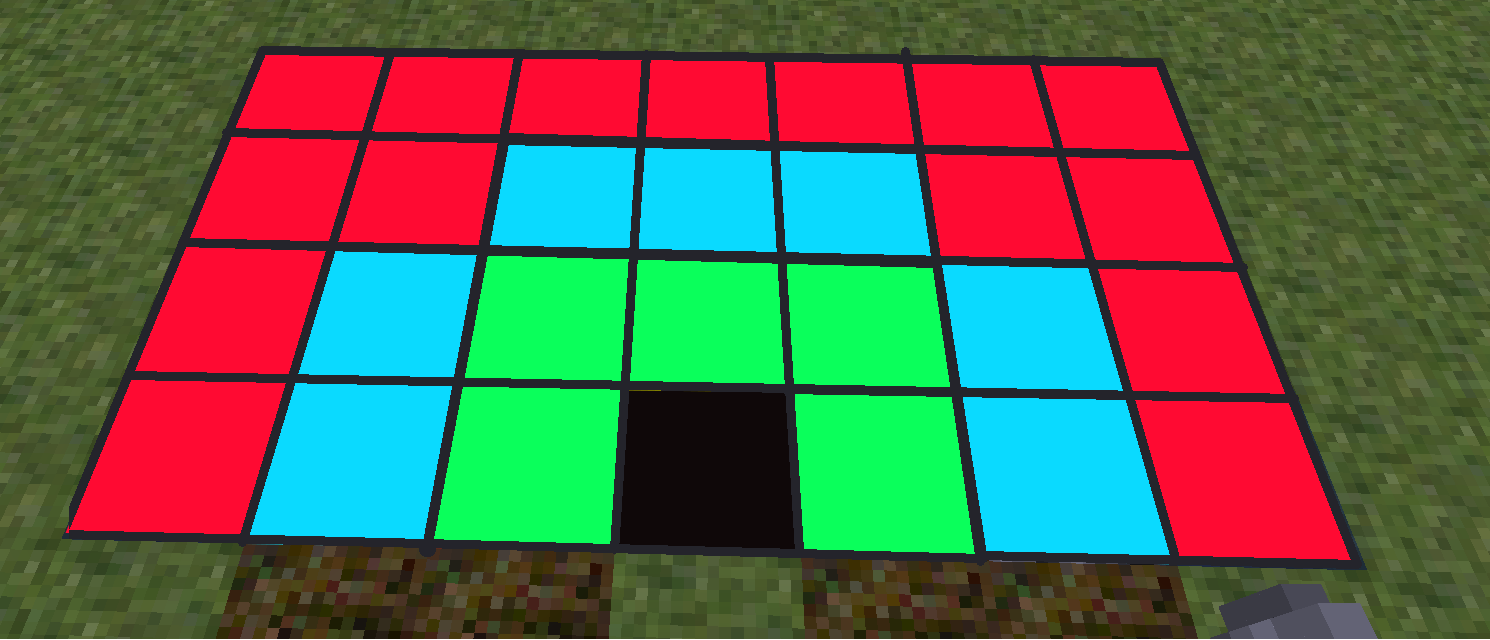
\includegraphics[scale=0.25]{src/lava_runner/res/1layer.png}
\caption{Das schwarz markierte Feld stellt die Position des vorherigen Blocks dar, die roten Felder sind nicht erreichbar, weshalb ein Block verworfen werden soll, falls er zufällig auf diesem Feld platziert werden soll.}
\end{figure}

\end{document}